\section{Architekturüberblick und Integration}

Die Abbildung \ref{fig:feasibility-check-komponentendiagramm} veranschaulicht die erweiterte REALIS-Architektur zur Realisierung des Feasibility Checks. Basierend auf dem bestehenden REALIS-Komponenten\-diagramm (siehe Abbildung 2.3) werden neue Komponenten hinzugefügt, um die Feasibility-Check-Funktionalität zu integrieren. Im Diagramm sind dabei aus Gründen der Übersichtlichkeit nur die wichtigsten Erweiterungen dargestellt.

\begin{figure}[!htbp]
    \centering
    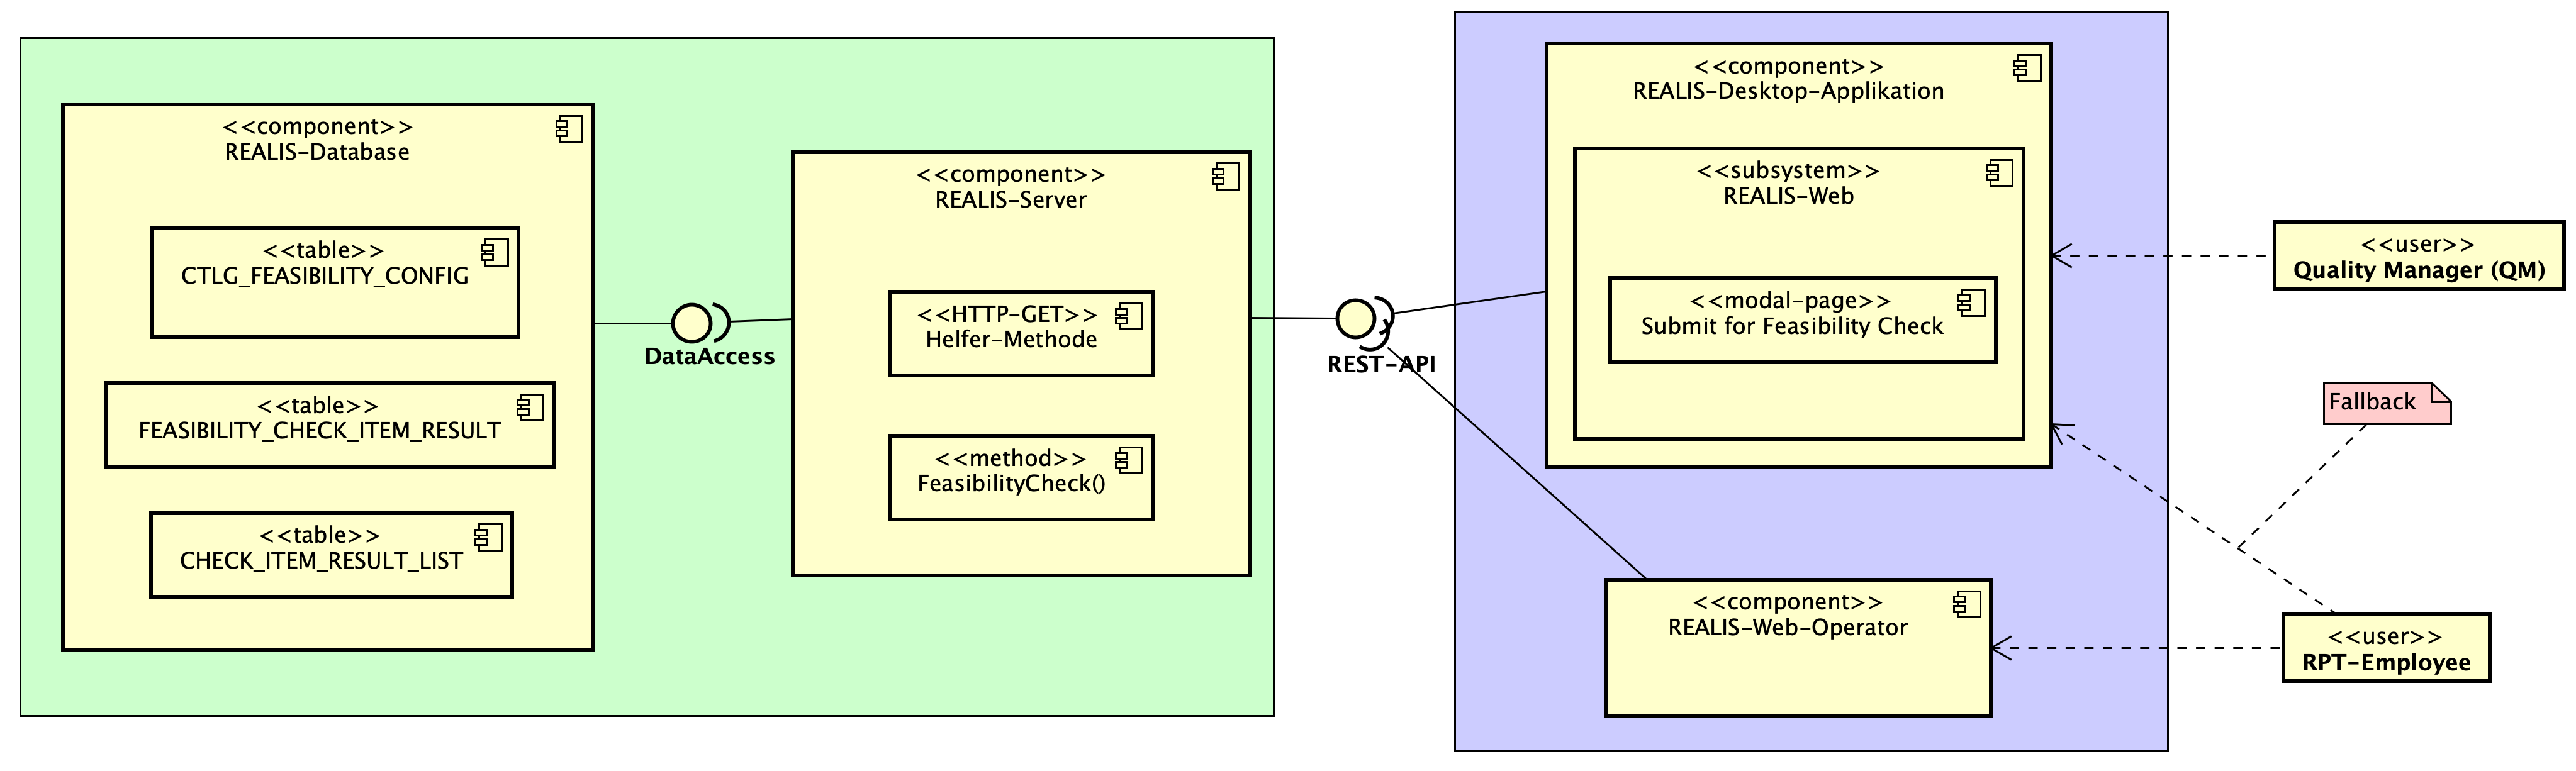
\includegraphics[width=1\textwidth]{bilder/REALIS-Komponentendiagramm-mit-Erweiterungen2.png}
    \caption{Feasibility Check Architekturdesign-Erweiterung von \gls{REALIS}}
    \label{fig:feasibility-check-komponentendiagramm}
\end{figure}



In der \textbf{Datenbank} werden neue Tabellen hinzugefügt, die sowohl zur Konfiguration als auch zur Speicherung der Feasibility Check Ergebnisse dienen. Hierzu gehören die Tabellen \texttt{ctlg\_feasibility\_config}, \texttt{feasibility\_check\_item\_result} und \texttt{check\_item\_\-result\_\-list}.

Im \textbf{Backend} wird eine HTTP-GET-Methode (in Abb. \ref{fig:feasibility-check-komponentendiagramm} und \ref{fig:sequence-diagram} mit ''Helfer-Methode'' benannt) implementiert. Diese Methode ruft den Kern-Algorithmus, die Funktion \texttt{FeasibilityCheck()} auf, die die eigentliche Datenverarbeitung übernimmt, die Ergebnisse der Feasibility Check Überprüfung in der Datenbank abspeichert und diese über die ''Helfer-Methode'' an das Frontend liefert.

Im \textbf{Frontend} wird im \textit{REALIS-Web Subsystem} eine neue Modal-Page ''Submit for Feasibility Check'' integriert, die es Benutzern ermöglicht, den Feasibility Check zu initiieren. Nach der Überprüfung werden die Ergebnisse übersichtlich dargestellt und zusätzliche Details können bei Bedarf abgerufen werden. 

Durch diese Erweiterungen wird die Feasibility-Check-Funktion nahtlos in die bestehende REALIS-Architektur eingebettet und ermöglicht eine effiziente Interaktion mit den relevanten Benutzern und Systemkomponenten.

Die wichtigsten Interaktionen zwischen Benutzer (\gls{QM}), Frontend, Backend und der Datenbank sind im Sequenzdiagramm in Abbildung \ref{fig:sequence-diagram} dargestellt. Die einzelnen Komponenten werden in den folgenden Kapiteln detailliert beschrieben. 

\begin{figure}[!htbp]
    \centering
    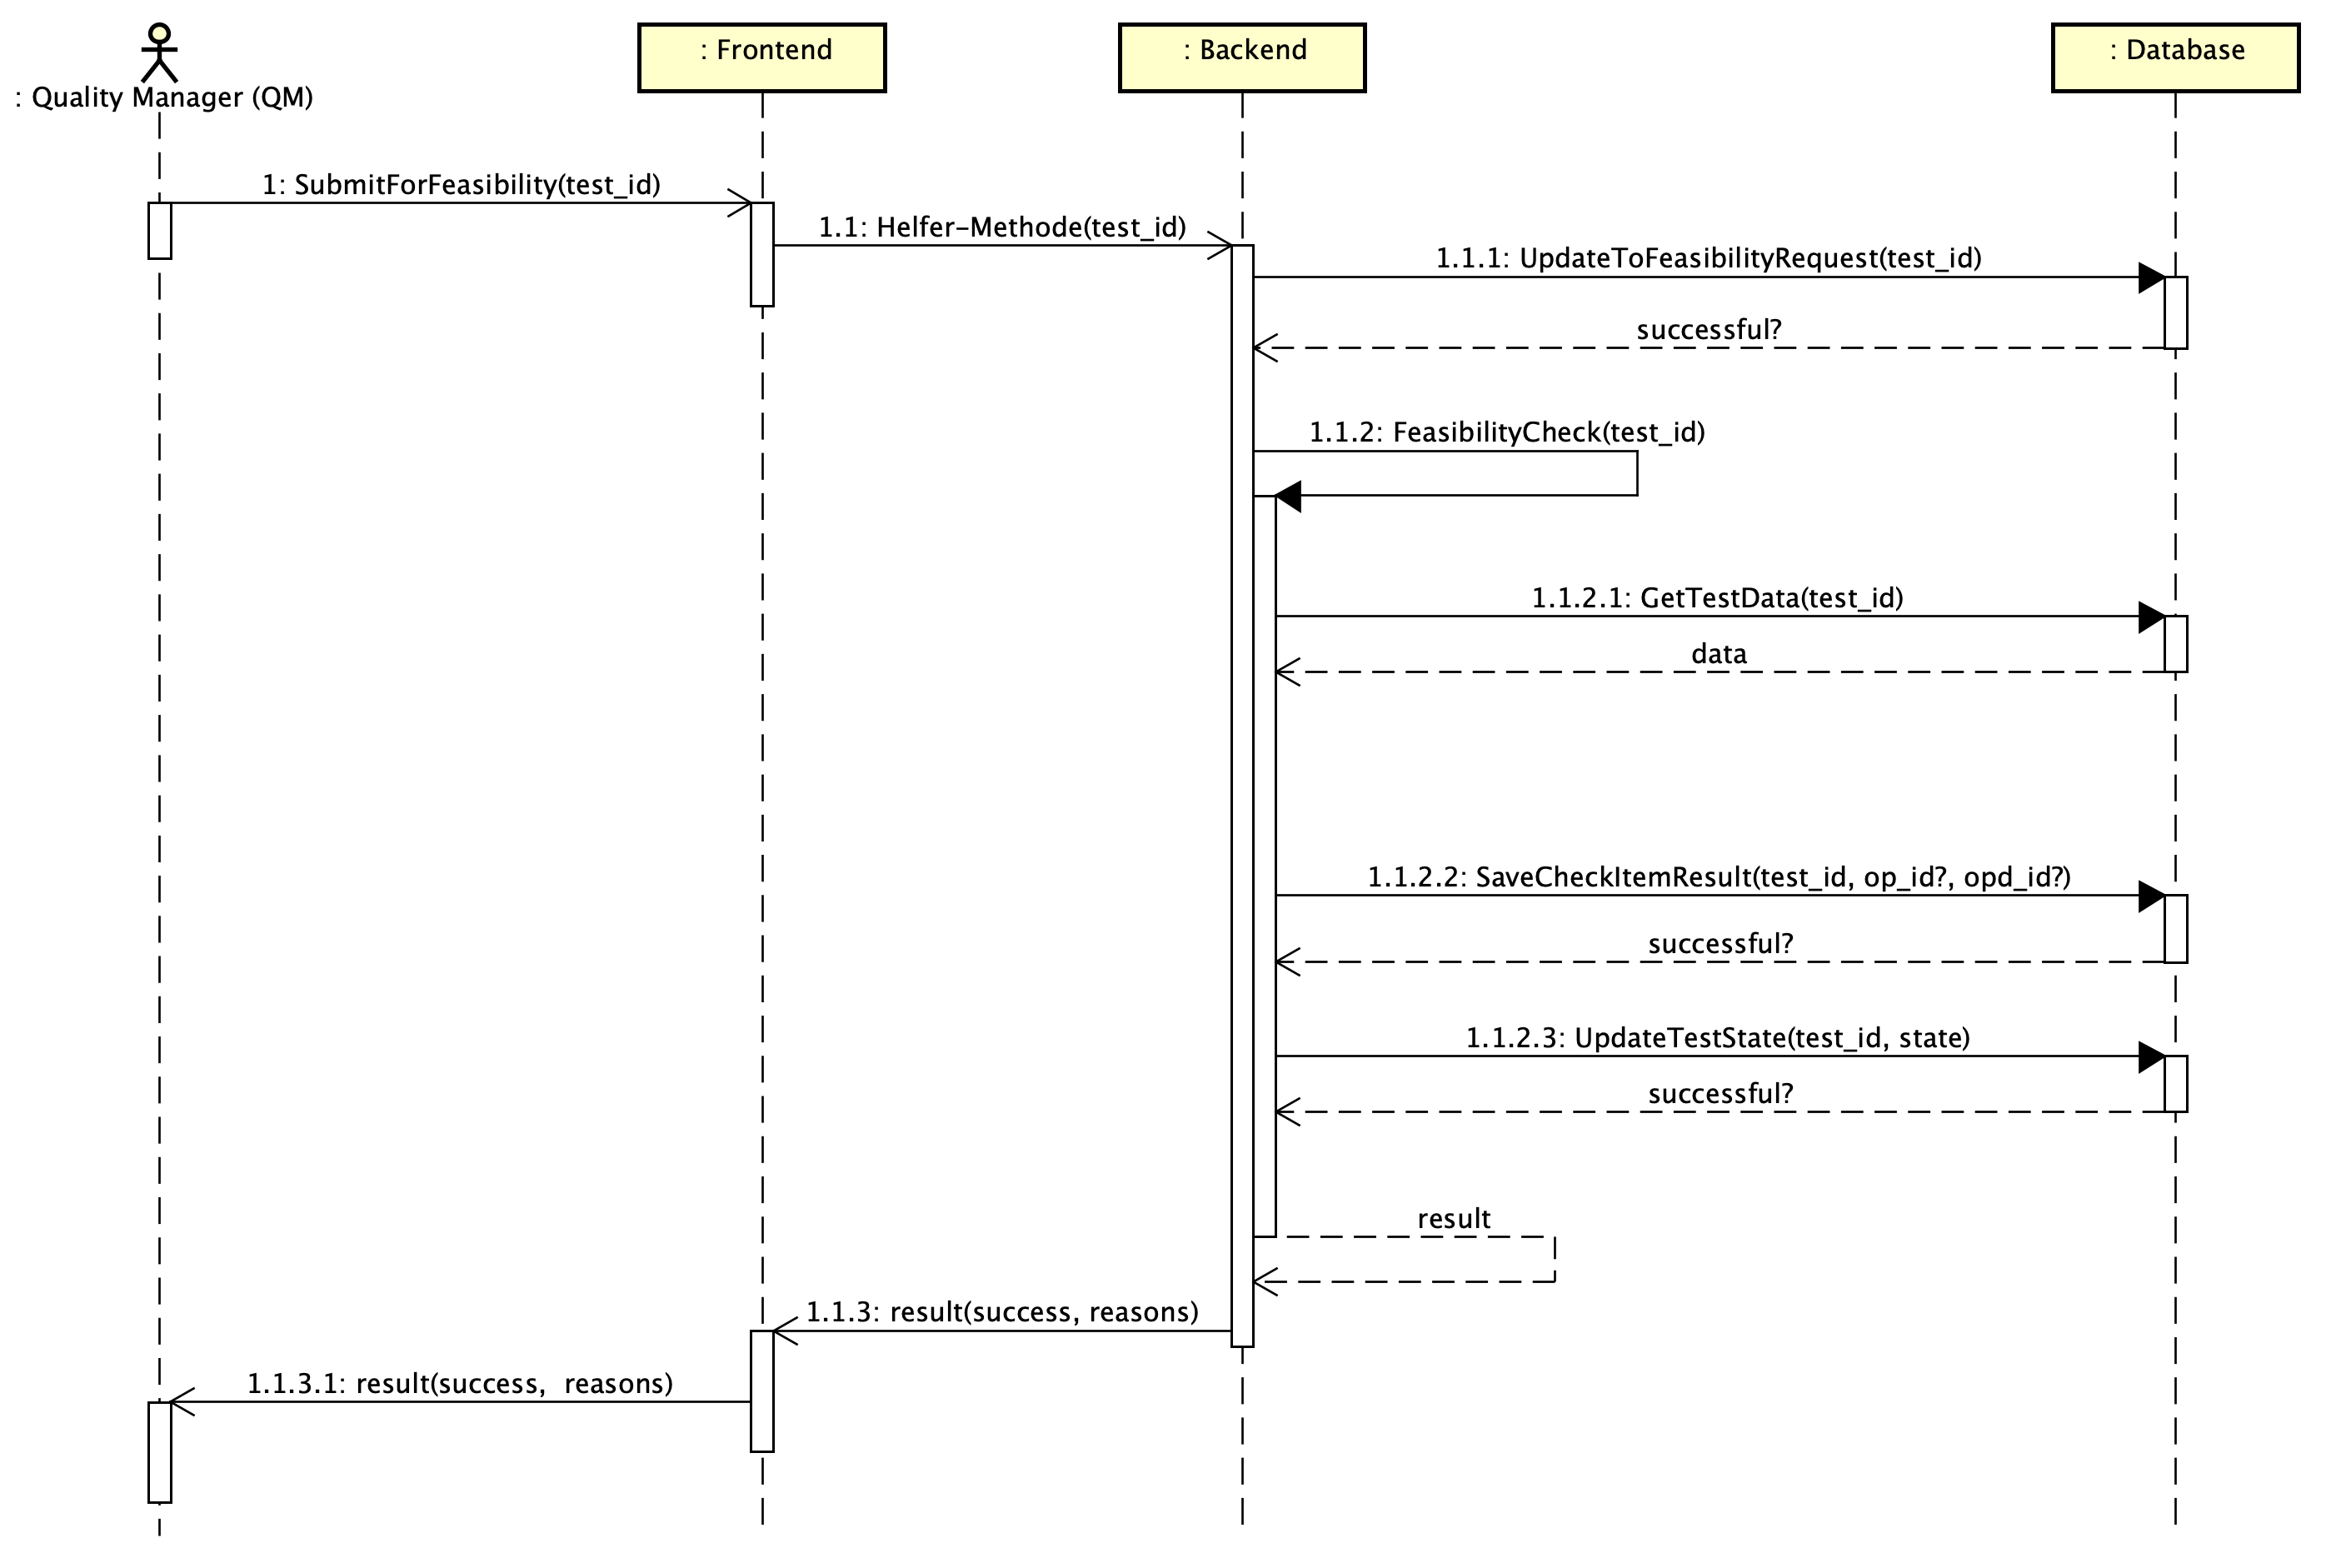
\includegraphics[width=1\textwidth]{bilder/Feasibility-Sequenz-Diagramm.png}
    \caption{Sequenzdiagramm Feasibility Check}
    \label{fig:sequence-diagram}
\end{figure}


